% small.tex
\documentclass{beamer}
\usetheme{Boadilla}
\setbeamertemplate{blocks}[rounded][shadow=false] 

\usepackage{subfig}
\usepackage{multirow}
\usepackage{amsmath}
\usepackage{mathtools}
\usepackage{listings}
\usepackage{color}
\usepackage{multirow}
\usepackage{pifont}% http://ctan.org/pkg/pifont
\newcommand{\starmark}{\ding{104}}%
\usepackage{bm}
\usepackage{colortbl}
 
\definecolor{periwinkle}{rgb}{0.6,0.6,1}
\definecolor{dkgreen}{rgb}{0,0.6,0}
\definecolor{gray}{rgb}{0.5,0.5,0.5}
\definecolor{mauve}{rgb}{0.58,0,0.82}

\lstset{ %
  language=Python,                % the language of the code
  basicstyle=\footnotesize,           % the size of the fonts that are used for the code
  %numbers=left,                   % where to put the line-numbers
  %numberstyle=\tiny\color{gray},  % the style that is used for the line-numbers
  %stepnumber=2,                   % the step between two line-numbers. If it's 1, each line 
                                  % will be numbered
  %numbersep=5pt,                  % how far the line-numbers are from the code
  %backgroundcolor=\color{white},      % choose the background color. You must add \usepackage{color}
  showspaces=false,               % show spaces adding particular underscores
  showstringspaces=false,         % underline spaces within strings
  showtabs=false,                 % show tabs within strings adding particular underscores
  %frame=single,                   % adds a frame around the code
  rulecolor=\color{black},        % if not set, the frame-color may be changed on line-breaks within not-black text (e.g. commens (green here))
  tabsize=2,                      % sets default tabsize to 2 spaces
  captionpos=b,                   % sets the caption-position to bottom
  breaklines=true,                % sets automatic line breaking
  breakatwhitespace=false,        % sets if automatic breaks should only happen at whitespace
  title=\lstname,                   % show the filename of files included with \lstinputlisting;
                                  % also try caption instead of title
  keywordstyle=\color{blue},          % keyword style
  commentstyle=\color{dkgreen},       % comment style
  stringstyle=\color{mauve},         % string literal style
  escapeinside={\%*}{*)},            % if you want to add a comment within your code
  morekeywords={dynamic, string}               % if you want to add more keywords to the set
}


\AtBeginSection[]
{
  \begin{frame}
    \tableofcontents[currentsection]
  \end{frame}
}


%About me
\author{Wesley Brooks} 
\title{Modeling PalEON biomass}
%\subtitle{Wesley Brooks} 
\institute{UW-Madison} 

\begin{document}

%Title slide
\begin{frame}
  \titlepage
\end{frame}


%Table of contents
\begin{frame}{Outline}
  \tableofcontents
\end{frame}


%Goal
\begin{frame}{Goal}
  \begin{itemize}
    \item Produce a model of per-species biomass at time of settlement
    \item Complicated by the presence of zeros
  \end{itemize}
\end{frame}

\section{Data}

\begin{frame}{Most common taxa}
	% latex table generated in R 2.15.2 by xtable 1.7-0 package
	% Mon May 27 19:31:33 2013
	\begin{table}[ht]
	\begin{center}
	\begin{tabular}{rr}
	  \textbf{Taxon} & \textbf{Biomass} \\
	  \rowcolor[gray]{0.9}Oaks & 7900000 \\ 
	  Pine & 6900000 \\ 
	  Hemlock & 6500000 \\ 
	  Birches & 6400000 \\ 
	  \rowcolor[gray]{0.9}Maple & 4900000 \\ 
	  Basswood & 1700000 \\ 
	  Elms & 1600000 \\ 
	  Tamarack & 1600000 \\ 
	  Cedar & 1500000 \\ 
	\end{tabular}
	\end{center}
	\end{table}
\end{frame}

%Oaks
\begin{frame}{Oaks}
\begin{center}
  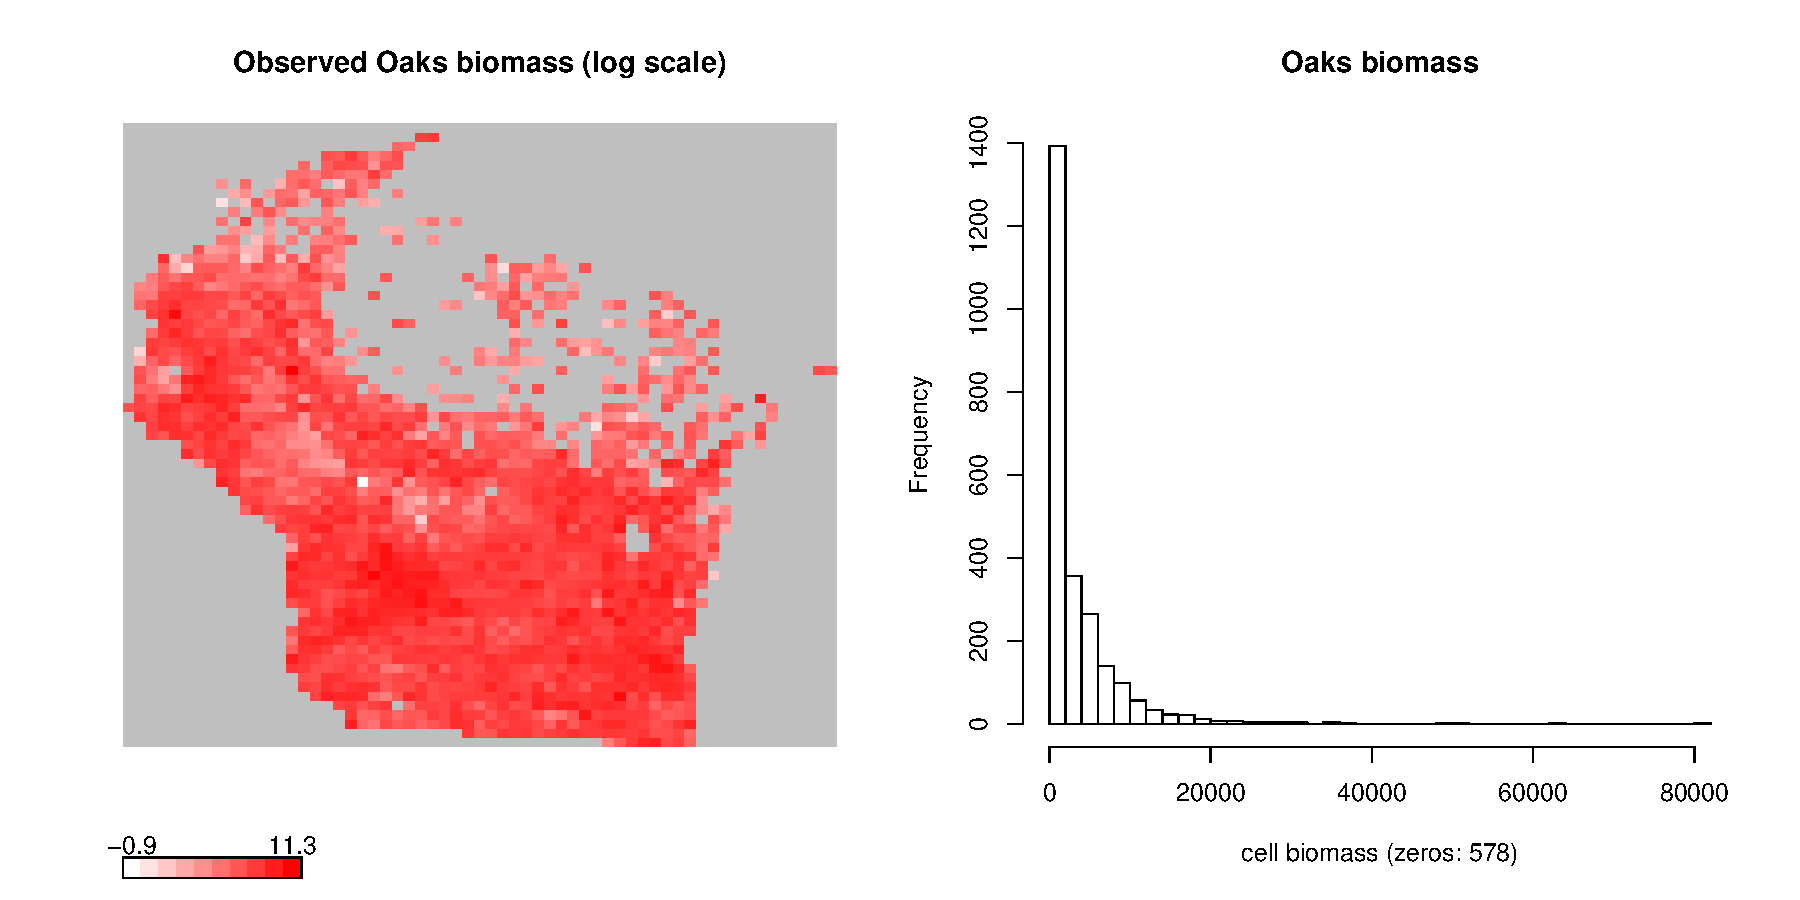
\includegraphics[width=\textwidth]{../../figures/raw/Oaks-observed-heatmap.pdf}
\end{center}
\end{frame}

%Pine
\begin{frame}{Pine}
\begin{center}
  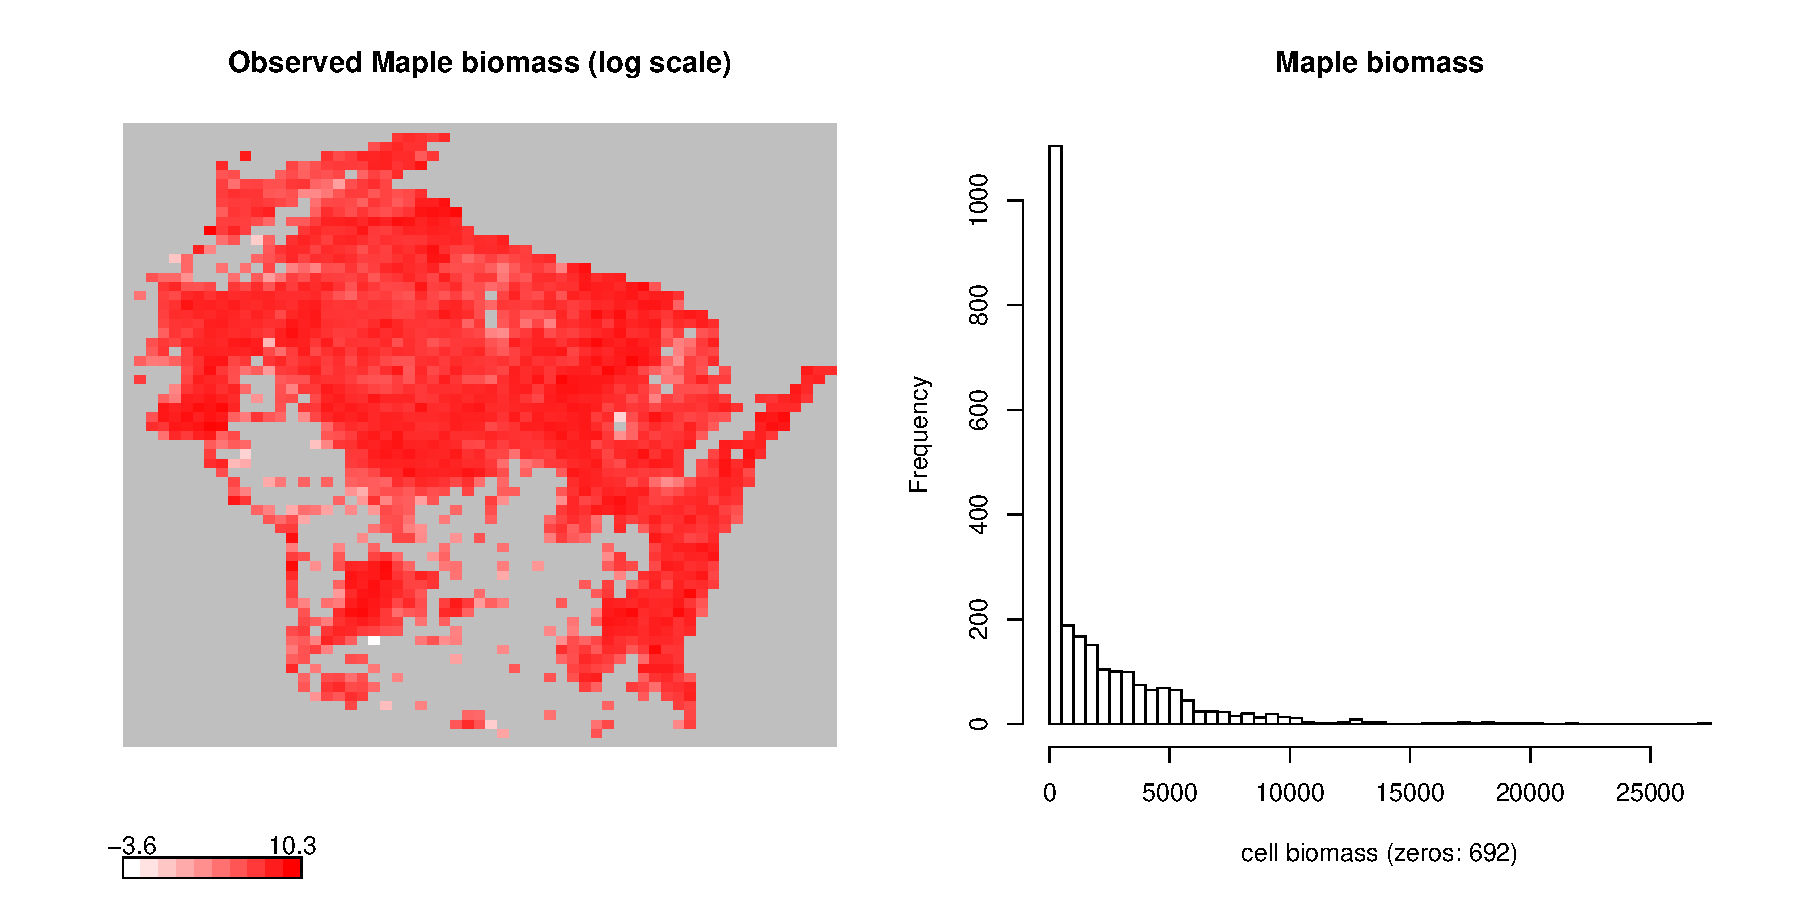
\includegraphics[width=\textwidth]{../../figures/raw/Maple-observed-heatmap.pdf}
\end{center}
\end{frame}

%Biomass vs composition
\begin{frame}{}
  \begin{center}
    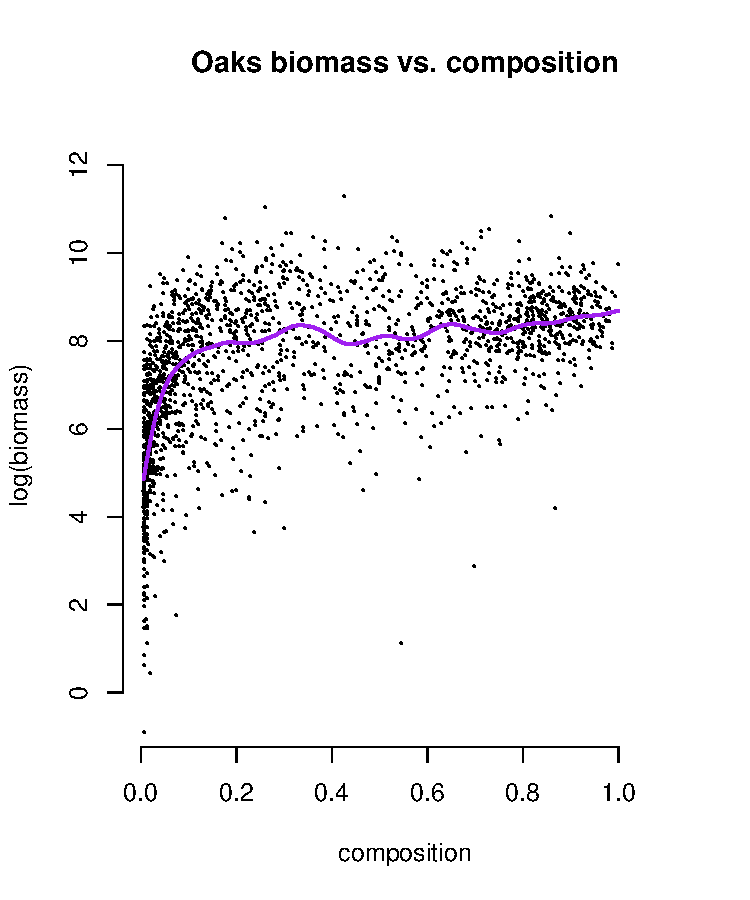
\includegraphics[width=0.45\textwidth]{../../figures/raw/Oaks-biomass-v-composition.pdf}
    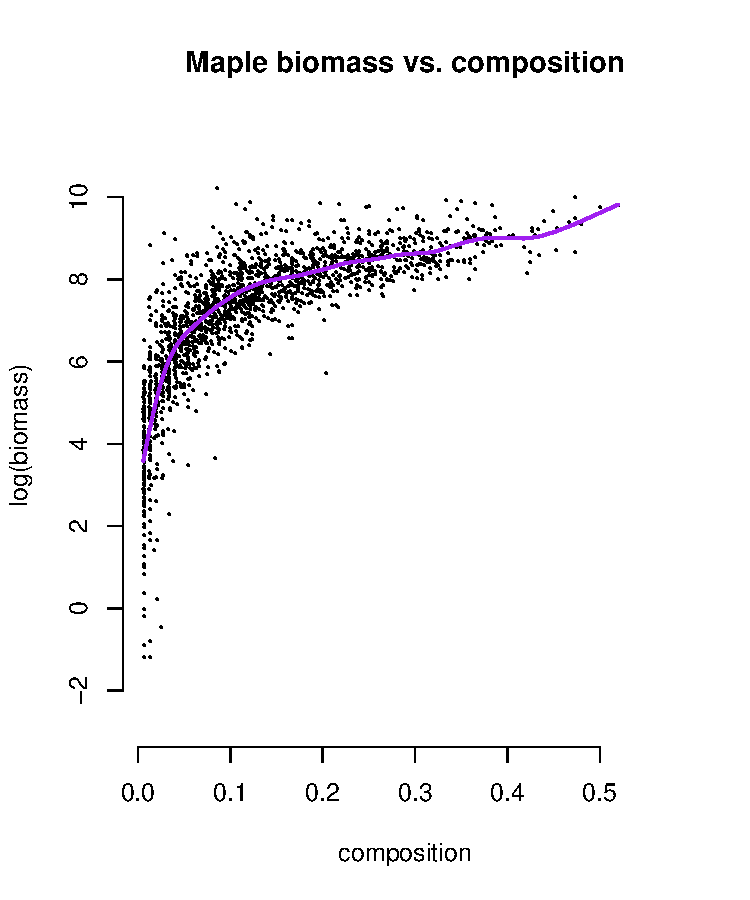
\includegraphics[width=0.45\textwidth]{../../figures/raw/Maple-biomass-v-composition.pdf} 
  \end{center}
\end{frame}


\section{Modeling}

%Modeling matrix
\begin{frame}{Modeling grid}
  \begin{center}
    \begin{tabular}{c|c|r|c|c|c|}
    \multicolumn{2}{c}{} & \multicolumn{3}{c}{Spatial fit}\\
    \multicolumn{2}{c}{} & \multicolumn{1}{c}{\rotatebox{60}{Indep.}} & \multicolumn{1}{c}{\rotatebox{60}{Splines}} & \multicolumn{1}{c}{\rotatebox{60}{GMRF}}\\
    \cline{2-5}
    \multirow{2}{*}{\rotatebox{90}{Model}}  & One-stage (Tweedie) &  &  & \\
    \cline{2-5}
    & Two-stage (Bernoulli-Gamma) & & & \\
    \cline{2-5}
    \end{tabular}
  \end{center}
\end{frame}
   
   
%More about the models/fitting methods
\begin{frame}
  \begin{itemize}
    \item Model types:
    \begin{itemize}
      \item Tweedie: single stage model that accounts for exact zeros
      \item Binomial-Gamma: binomial stage for presence/absence and gamma stage for biomass, conditional on presence
    \end{itemize}
    \item Spatial fitting methods:
    \begin{itemize}
      \item Independent: ignore spatial structure, treat observations as conditionally independent
      \item Splines: smoothing spline for the spatial effect
      \item GMRF: spatial random effect (fit with the INLA algorithm)
    \end{itemize}
  \end{itemize}
\end{frame}


\begin{frame}{Defining terms}
  Let:
  \begin{itemize}
    \item $s$ index location, $k$ index taxon\\
    \item $Y_{k,s}$ denote the biomass of taxon $k$ in cell $s$\\
    \item $p_{k,s}$ denote the composition fraction of taxon $k$ in cell $s$\\
    \item $\gamma_s$ denote the overall stem density in grid cell $s$
  \end{itemize}
\end{frame}

\section{Model structure}

\subsection{Two-stage}

  %Model types
\begin{frame}[fragile]{Two-stage models}
  \begin{itemize}
    \item First stage: zero/non-zero
    \begin{itemize}
      \item Logistic regression
      \item $Z_s \sim \text{Bernoulli}(\zeta_s)$
      \item $\text{logit}(\zeta_s) = f(\cdots)$
    \end{itemize}
    \item Second stage: distribution of positive biomass
    \begin{itemize}
      \item $Y_s|Z_s=1 \sim \text{Gamma}(\alpha_s, \beta_s)$
      \item $\text{E}\left(Y_s|Z_s=1\right) = \mu_s = g(\eta_s)$
      \item $\eta_s = h(\cdots)$
    \end{itemize}
  \end{itemize}
\end{frame}


\subsection{One-stage}

  %Models
\begin{frame}[fragile]{One-stage models: the Tweedie family}
  \begin{itemize}
    \item Tweedie-family distributions have a point mass at zero as well as a continuous positive distribution.\\
    \item Parameter $\theta$ controls the mixture, from $\theta$ = 1 (Poisson) to $\theta$ = 2 (Gamma)
  \end{itemize}
  \begin{center}
      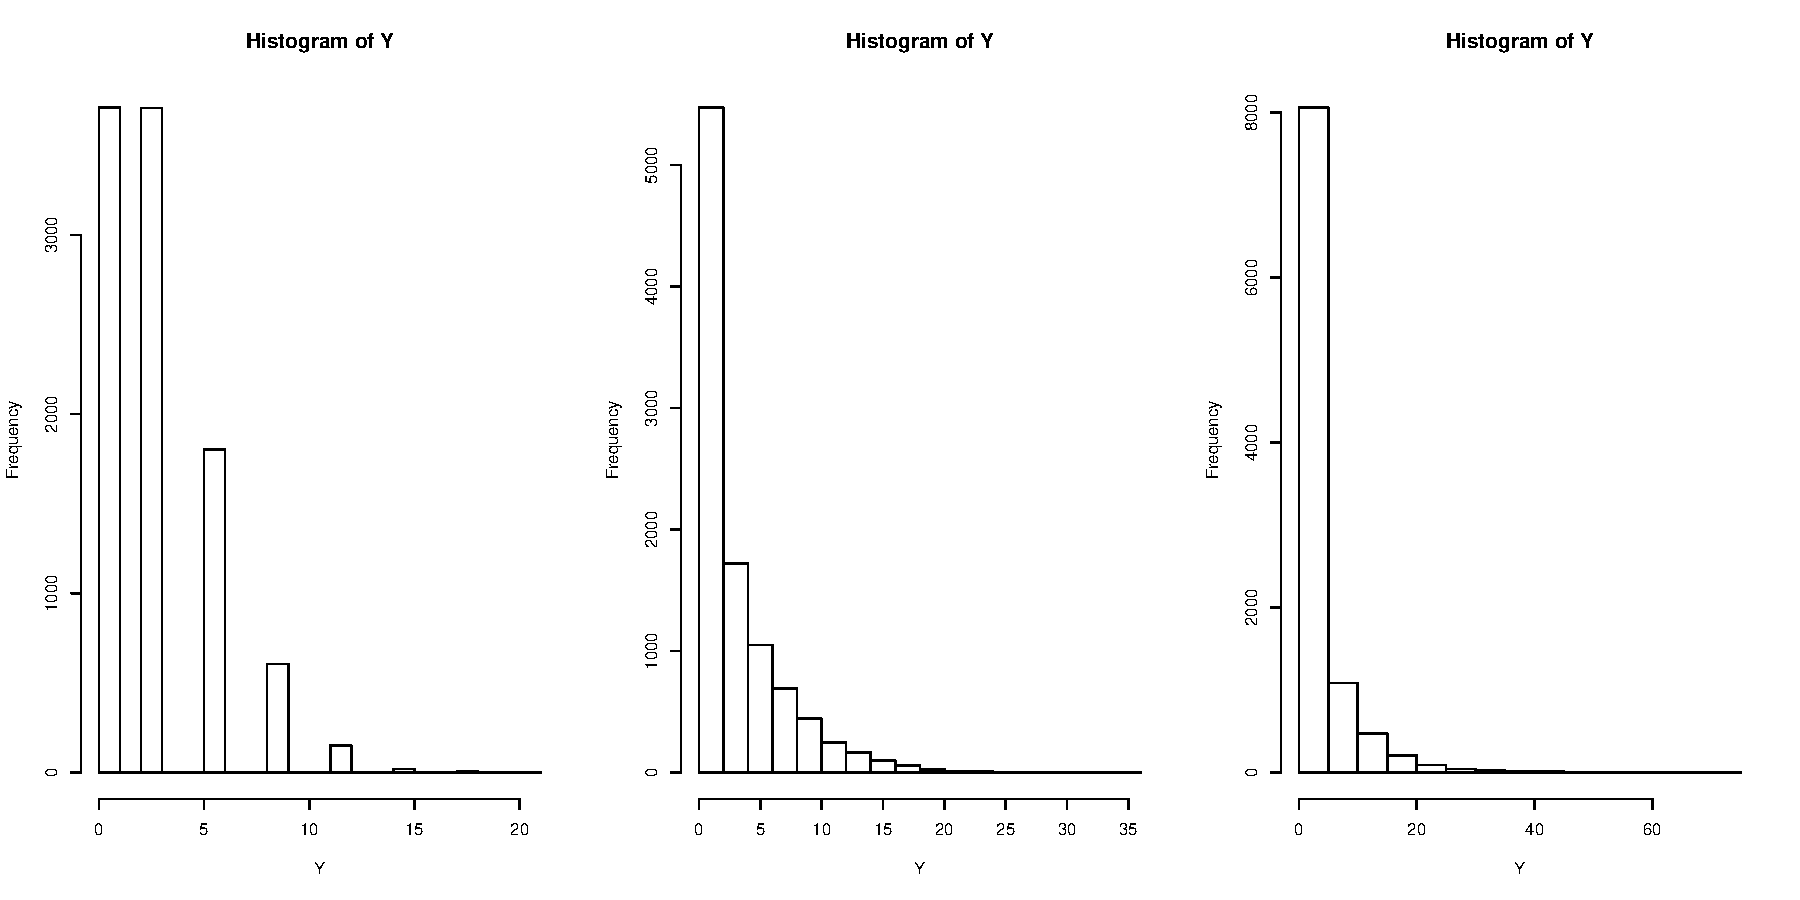
\includegraphics[width=0.9\textwidth]{../../figures/tweedie-sim.pdf}
  \end{center}
\end{frame}  

\begin{frame}
  Conceptualizing the Tweedie distribution as a Gamma-Poisson mixture with parameters $\alpha$, $\beta$, and $\lambda$:\\
  \begin{itemize}
    \item Draw $N \sim \text{Poisson}(\lambda)$
    \item Now make $N$ iid draws: $V_{\ell} \sim \text{Gamma}(\alpha, \beta)$
    \item $Y = \sum\limits_{\ell=1}^N  V_{\ell}$
  \end{itemize}
\end{frame}


\begin{frame}[fragile]{Tweedie model}
  With $\theta$ given, the Tweedie distribution is in the exponential family.\\
  \begin{itemize}
    \item $EY = \mu$
    \item var$(Y) = \phi \mu^\theta$
    \item $\phi$ is a scale parameter
    \item $P(Y=0) = \exp{\left(-\phi^{-1} \frac{\mu^{2-\theta}}{2-\theta}\right)}$
    \begin{itemize}
      \item $P(Y=0) \uparrow$ as $\mu \rightarrow -\infty$
      \item $P(Y=0) \uparrow$ as $\phi \uparrow$
      \item $P(Y=0) \uparrow$ as $\theta \rightarrow 1$
    \end{itemize}
    \item But we first need $\theta$
    \begin{itemize}
      \item Find $\hat{\theta}$ so that the model's deviance residuals match the assumed variance function. 
    \end{itemize}
  \end{itemize}
\end{frame}


\section{Spatial fitting}

\subsection{Independent grid cells}

\begin{frame}{Independent grid cells}
  Ignoring the spatial structure, model the biomass as a function of composition and stem density\\
  \begin{align*}
    \eta_s &= f(p_{k,s}, \gamma_s)\\
    \mu_s &= EY_s = \exp{(\eta_s)}\\
    Y_s &\sim \text{Tweedie}(\mu_s, \theta)\\
  \end{align*}
  \begin{itemize}
    \item 
  \end{itemize}

\end{frame}

\begin{frame}
  The pictures are from a one-stage model for Maple:\\
  \begin{center}
    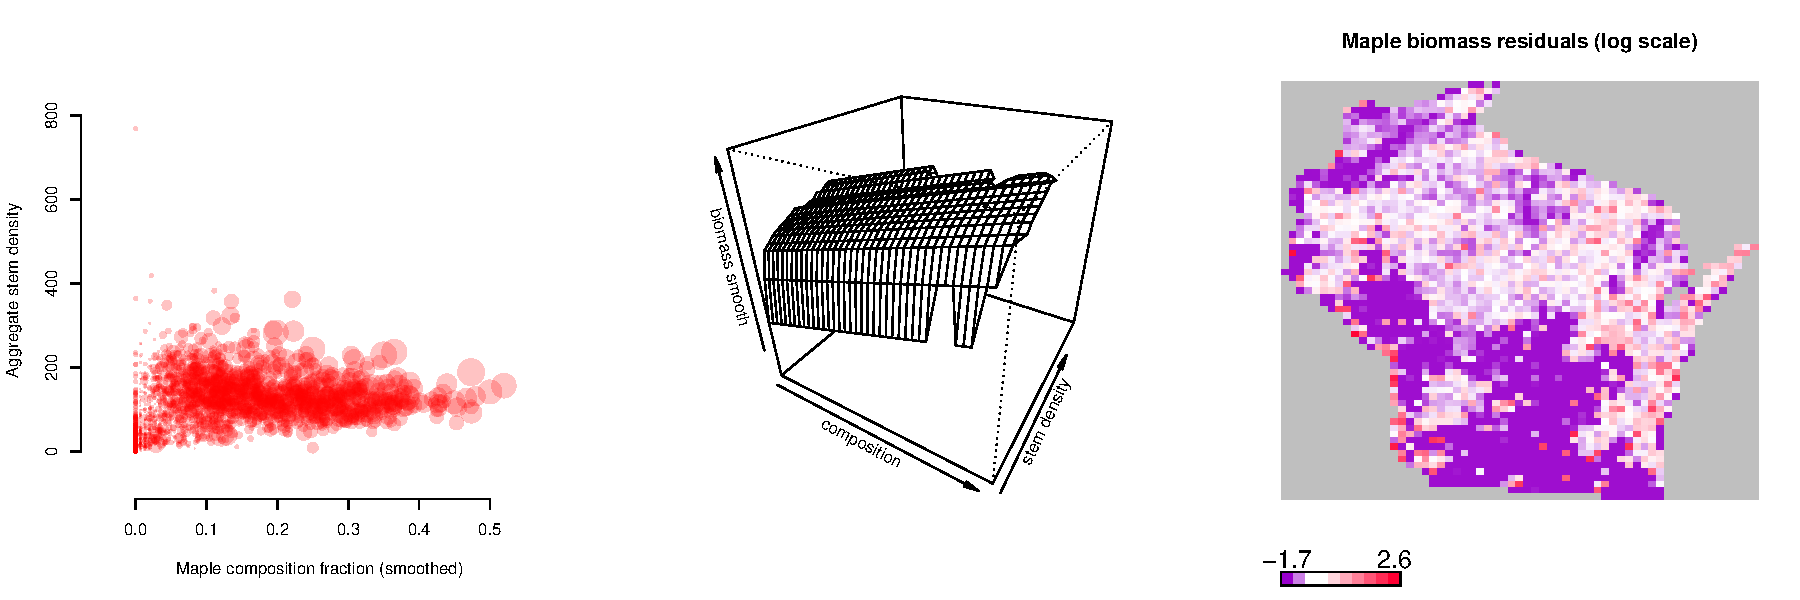
\includegraphics[width=0.9\textwidth]{../../figures/aspatial-tweedie/Maple-plots.pdf}
  \end{center}
\end{frame}

\begin{frame}{Independent grid cells}
 Pictures here are from a one-stage model for Oak.\\
  \begin{center}
    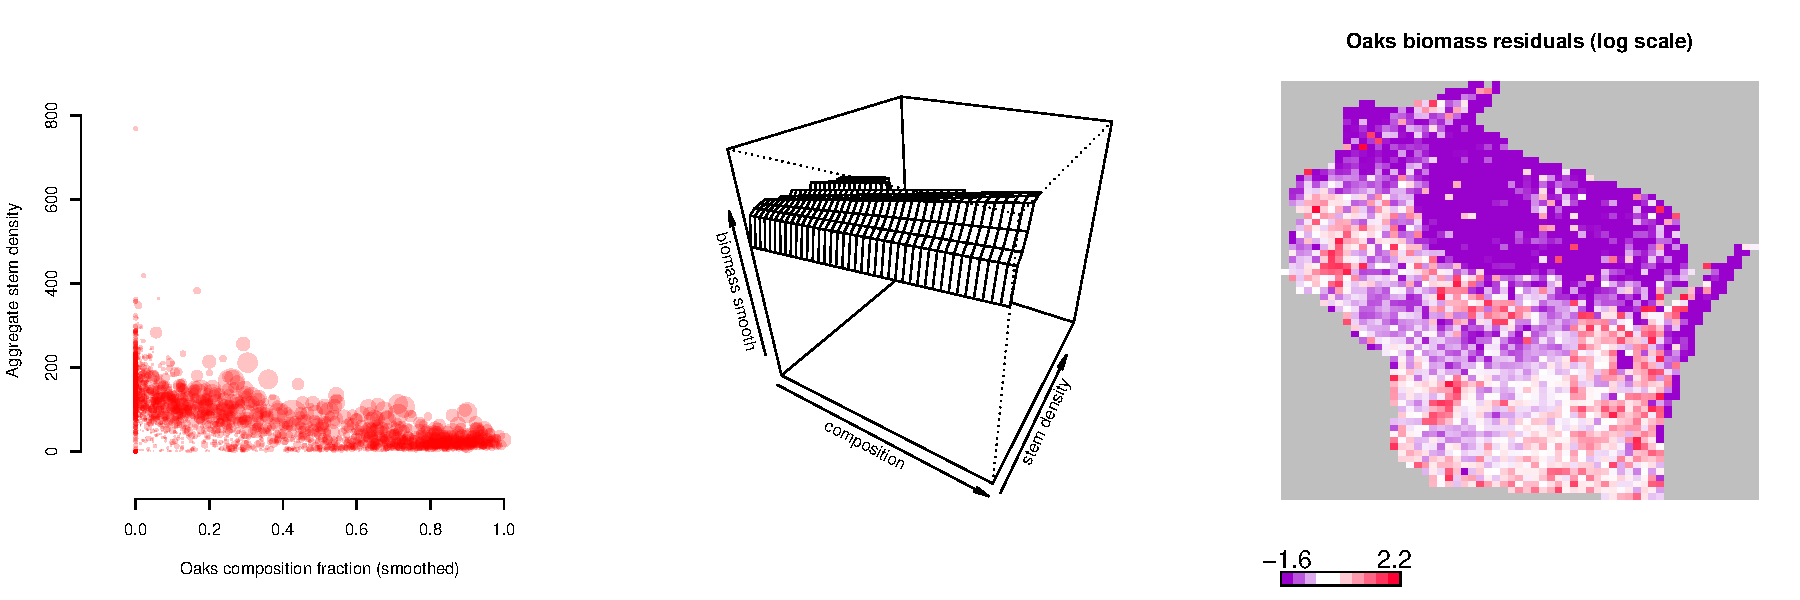
\includegraphics[width=0.9\textwidth]{../../figures/aspatial-tweedie/Oaks-plots.pdf}
  \end{center}
\end{frame}

\subsection{Spline models}
\begin{frame}{Spline models}
  One way to account for spatial patterns is by using splines to model a spatial effect. Essentially the splines are a smooth function of latitude and longitude, and are fit using the same software as was used for the smooth functions of composition and stem density in the independent grid cell models.
  
  \begin{align*}
      \eta_s &= f(p_{k,s}, \gamma_s) + g(s_x, s_y)\\
      \mu_s &= EY_s = \exp{(\eta_s)}\\
      Y_s &\sim \text{Tweedie}(\mu_s, \theta)\\
  \end{align*}
\end{frame}

\begin{frame}{Spline models - Maple}
 Pictures here are from a one-stage spline model for Maple.\\
  \begin{center}
    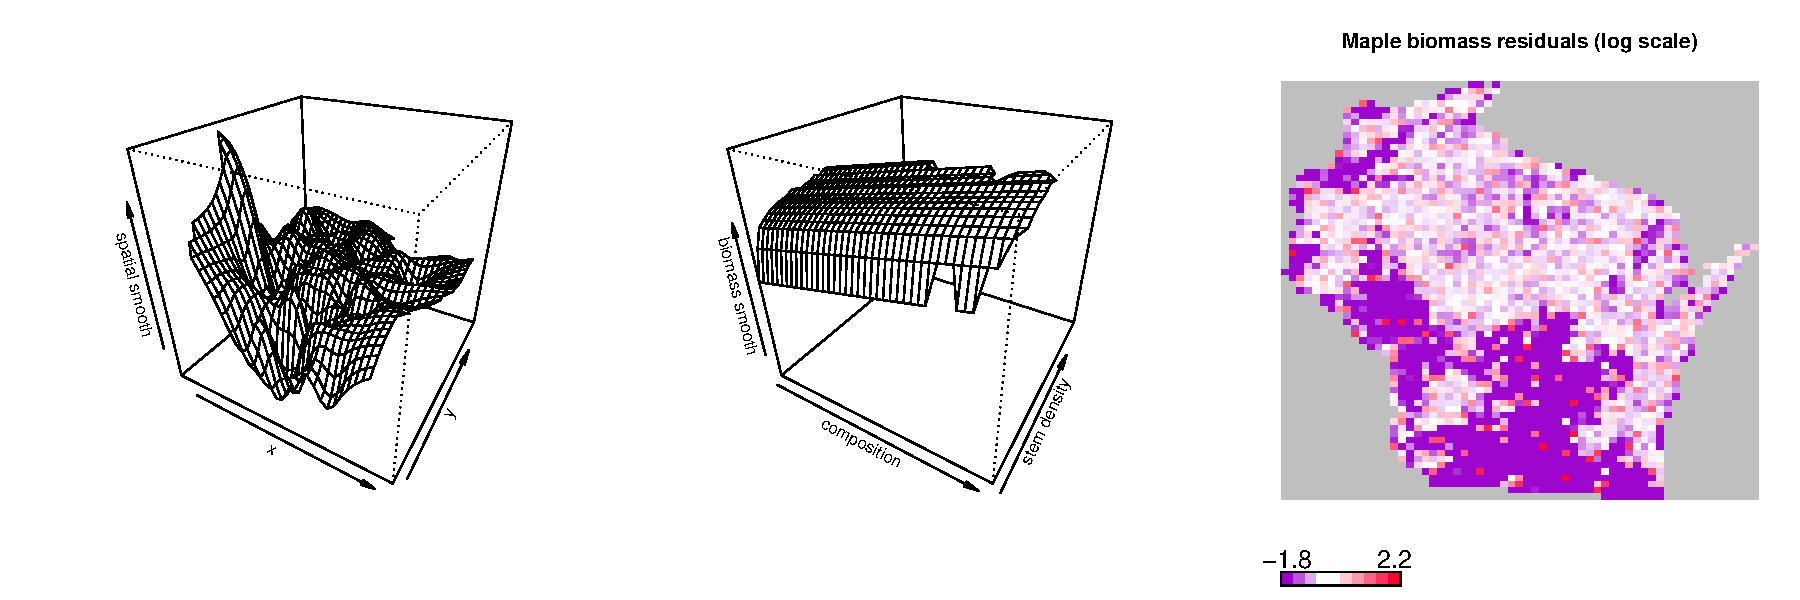
\includegraphics[width=0.9\textwidth]{../../figures/spline-tweedie/Maple-residuals-heatmap.pdf}
  \end{center}
\end{frame}

\begin{frame}{Independent grid cells}
 Pictures here are from a one-stage spline model for Oak.\\
  \begin{center}
    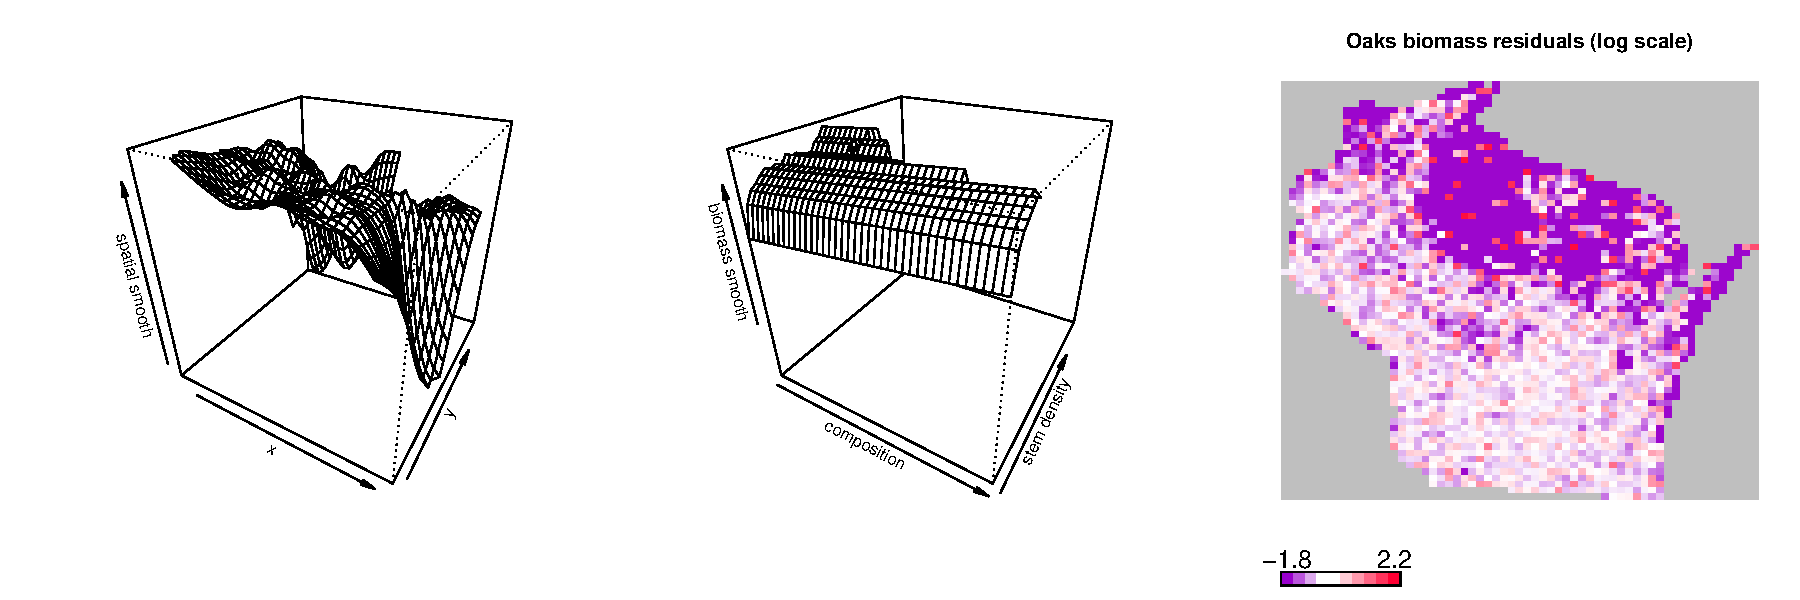
\includegraphics[width=0.9\textwidth]{../../figures/spline-tweedie/Oaks-residuals-heatmap.pdf}
  \end{center}
\end{frame}

\subsection{Bayesian hierarchical model}

\begin{frame}{Hierarchical model}
Consider a log-normal model where the mean is a Gaussian Process:
  \begin{align*}
    \log(Y_s) &\sim \mathcal{N} \left( g(s), \sigma^2 \right)\\
    g(\cdot) &\sim \text{GP}(f(\cdot), \Sigma)\\
  \end{align*}
  Parameters for such a Gaussian Process are often estimated by approximating it as a Gaussian Markov Random Field (GMRF)
\end{frame}


\begin{frame}{Gaussian Markov Random Field}
  \begin{itemize}
    \item Markov property says that all the relevant information for modeling a grid cell is found in its neighbors. 
    \item $g_i|\bm{g}_{-i}, \kappa \sim \mathcal{N}\left(n_i^{-1} \sum \limits_{j \in \partial_i} g_j, (n_i \kappa)^{-1}\right)$
  \end{itemize}
  
  \begin{center}
    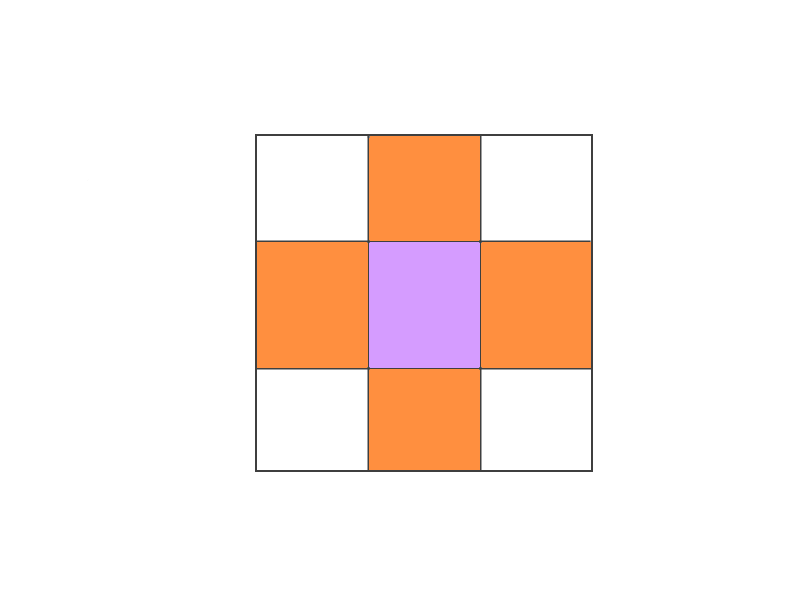
\includegraphics[width=0.4\textwidth]{../../figures/neighborhood.png}
  \end{center}  
\end{frame}

\begin{frame}
  The method of integrated Nested Laplace Approximations (INLA) can be used for parameter estimation, is much faster than MCMC. The INLA software can be used for two-stage models, but the Tweedie likelihood is not currently included.
  \begin{center}
    \includegraphics[width=0.9\textwidth]{../../figures/inla-delta/maple-fitted-heatmap.pdf}
  \end{center}
\end{frame}


\section{Methodological details}

%Modeling matrix
\begin{frame}{Modeling grid}
  \begin{center}
    \begin{tabular}{c|c|r|c|c|c|}
    \multicolumn{2}{c}{} & \multicolumn{3}{c}{Spatial fit}\\
    \multicolumn{2}{c}{} & \multicolumn{1}{c}{\rotatebox{60}{Indep.}} & \multicolumn{1}{c}{\rotatebox{60}{Splines}} & \multicolumn{1}{c}{\rotatebox{60}{GRF}}\\
    \cline{2-5}
    \multirow{2}{*}{\rotatebox{90}{Model}}  & One-stage (Tweedie) & \checkmark & \checkmark & \\
    \cline{2-5}
    & Two-stage (Bernoulli-Gamma) &\checkmark & \checkmark & \checkmark \\
    \cline{2-5}
    \end{tabular}
  \end{center}
\end{frame}

\section{Other}

\begin{frame}[fragile]
  \verb!COZIGAM!: an alternative for fitting the two-stage model
  \begin{itemize}
    \item COZIGAM stands for constrained zero-inflated GAM
    \item ``Constrained" means that the latent predictors for the $P(y=0)$ part and the $f(y|y>0)$ part must be proportional
    \item Package was removed from CRAN last year
    \item In testing with the archived version, algorithm convergence was elusive
  \end{itemize}
\end{frame}

\end{document}
